% 1977 年陕西卷第七题：P 为 △ABC 外一点，A′、B′、C′ 分别为 PA、PB、PC 的中点，
% 虚线为中点三角形 A′B′C′（按源卷第 3 页布局：P 左上、A 右上、B 左下、C 右下，C 带实心点）
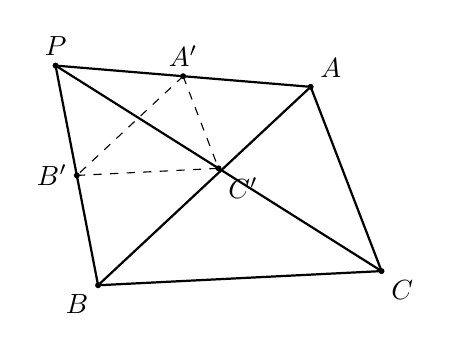
\begin{tikzpicture}[scale=0.9]
  \coordinate (P)  at (0,3.1);
  \coordinate (A)  at (3.6,2.8);
  \coordinate (B)  at (0.6,0);
  \coordinate (C)  at (4.6,0.2);
  \coordinate (Ap) at (1.8,2.95);
  \coordinate (Bp) at (0.3,1.55);
  \coordinate (Cp) at (2.3,1.65);
  \draw[thick] (P)--(A);
  \draw[thick] (P)--(B);
  \draw[thick] (P)--(C);
  \draw[thick] (A)--(B);
  \draw[thick] (B)--(C);
  \draw[thick] (A)--(C);
  \draw[dashed] (Ap)--(Bp);
  \draw[dashed] (Bp)--(Cp);
  \draw[dashed] (Ap)--(Cp);
  \fill (P)  circle (1.2pt) node[above] {$P$};
  \fill (A)  circle (1.2pt) node[above right] {$A$};
  \fill (B)  circle (1.2pt) node[below left] {$B$};
  \fill (C)  circle (1.2pt) node[below right] {$C$};
  \fill (Ap) circle (1.2pt) node[above] {$A'$};
  \fill (Bp) circle (1.2pt) node[left] {$B'$};
  \fill (Cp) circle (1.2pt) node[below right] {$C'$};
\end{tikzpicture}
